\section{Case Study}
\label{sec:case-study}

We consider a multi-hop network which has a chain of OpenWSN nodes (see Figure~\ref{fig:multihop}), and the {\em NodeId} (assigned as an integer) is increasing from left to right. 
\begin{figure}[t]
\centering
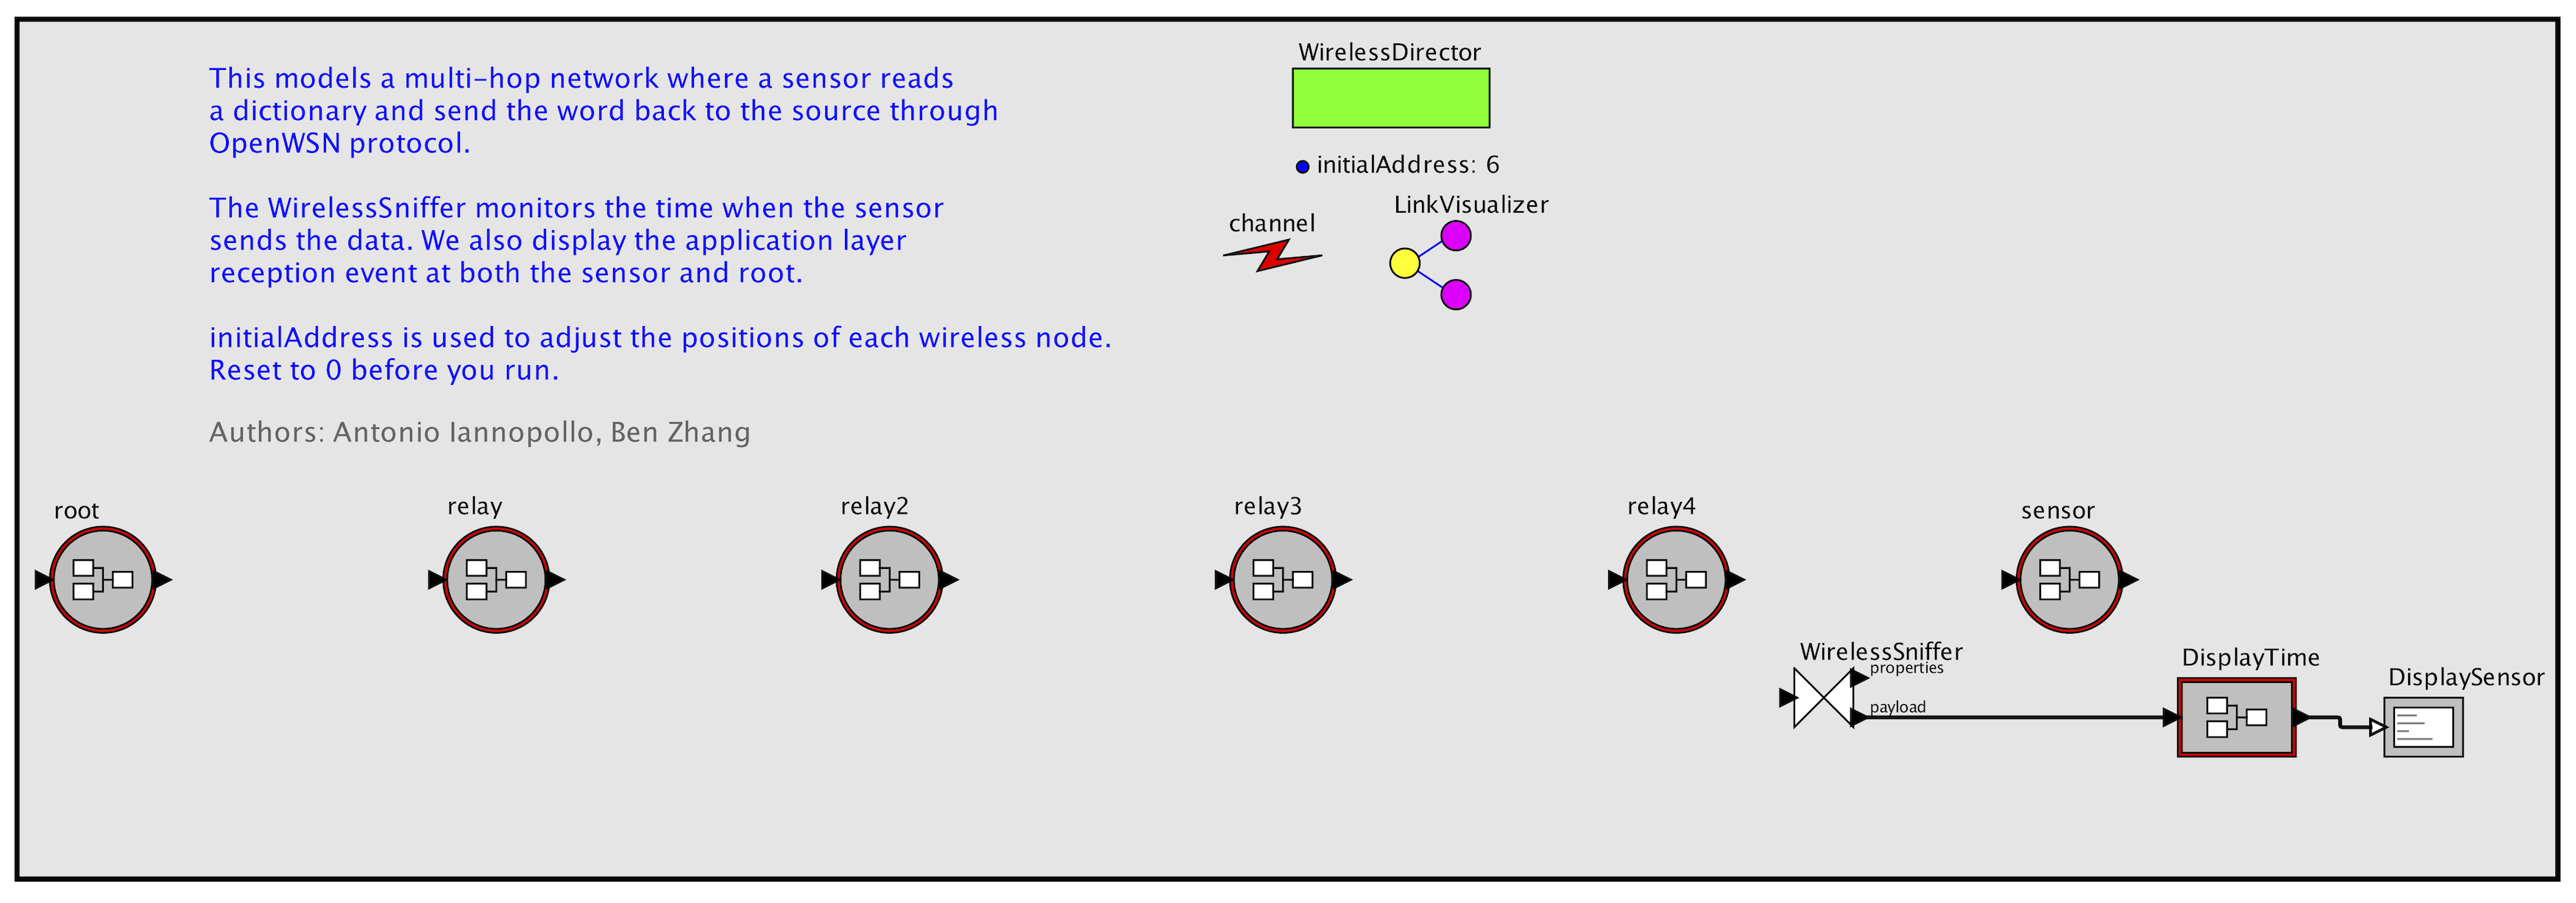
\includegraphics[width=1\columnwidth]{figures/PaperDemoPtolemy}
\caption{A multi-hop OpenWSN network.}
\label{fig:multihop}
\end{figure}
Their schedules are constructed in the following way\footnote{Interestingly, we are inspired by Gustove function to came up with such a schedule so that at any given time, a node is communicating only with one of its neighbors such that there will not be hidden terminal problem if time synchronization is achieved.}:

\begin{tabular}{ l | c | c | c | c | c }
  \hline                       
  NodeId & \multicolumn{5}{c}{Schedules} \\
  \hline
  $3i+0$ & \texttt{ADV} & \texttt{TX} & \texttt{RX} & \texttt{OFF} & $k \times \texttt{OFF}$ \\
  $3i+1$ & \texttt{ADV} & \texttt{RX} & \texttt{OFF} & \texttt{TX} & $k \times \texttt{OFF}$ \\
  $3i+2$ & \texttt{ADV} & \texttt{OFF} & \texttt{TX} & \texttt{RX} & $k \times \texttt{OFF}$ \\
  \hline  
\end{tabular}
where $i \in \mathbb{N}$ and $k$ is specified to control the duty cycle of each node (the number of \texttt{OFF} slots in the schedule; higher $k$ indicates lower duty cycle). Intuitively, when $k$ is small, nodes can receive \texttt{ADV} packet in a relatively timely fashion. This helps especially when they have lost synchronization. However, in this case the price they need to pay is to spend more time in \texttt{TX} and \texttt{RX} states, which potentially increases the power consumption. On the other hand, if $k$ is large, nodes that has lost synchronization will have to wait longer, leading to an increased energy consumption because of turning radio on and listening all the time. There might exist a {\em sweet point} of the duty cycle in this schedule pattern such that the overall energy consumption can be minimized. We leave a formal study as future work, and only focus on cases when $k = 0, 144, 306$ in this report.

\begin{figure}
\hfill
\subfigure[For each node, the time it first get synchronized (the time it joins the network).]{ 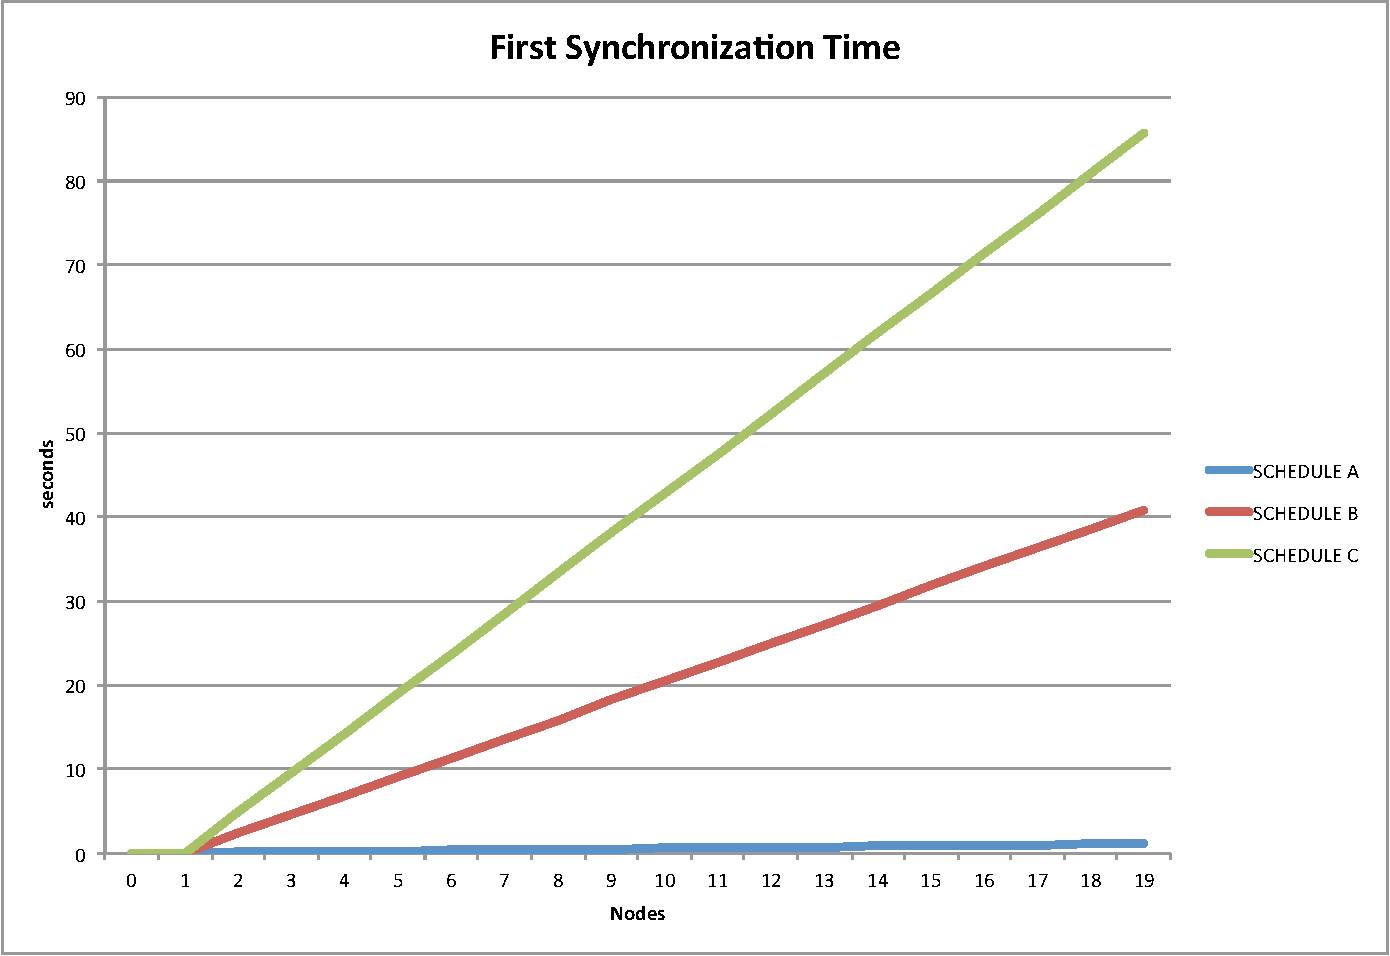
\includegraphics[width=.45\linewidth]{figures/synch_time_sched}}
\hfill
\subfigure[For each node, the measured power consumption after then network is on for 20 seconds.]{ 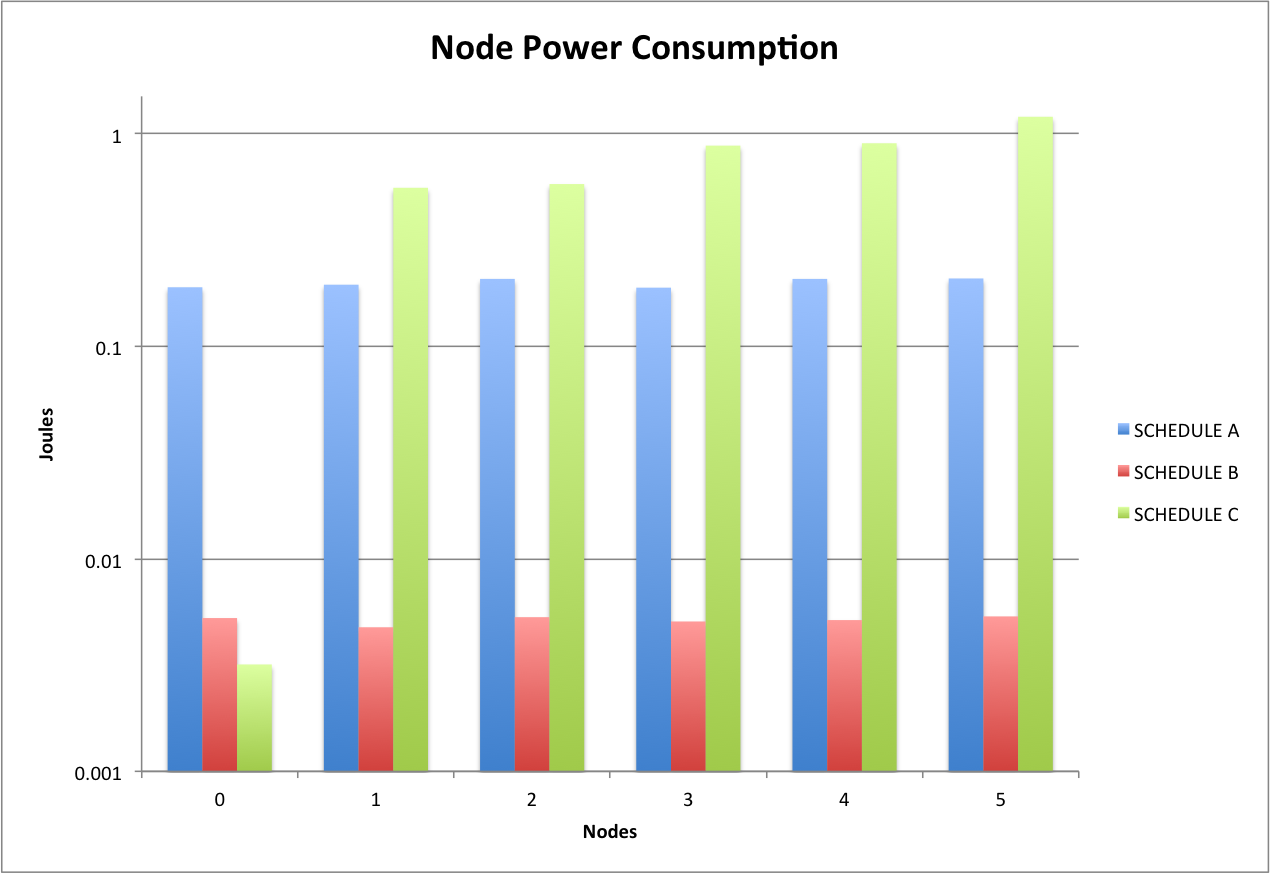
\includegraphics[width=.45\linewidth]{figures/power_cons}}
\hfill
\caption{Performance evaluation for different schedules in multi-hop network. Schedule A, B, C are corresponding to $k = 0, 144, 306$.}
\label{fig:evaluation}
\end{figure}

We present the results of a network that have 6 chained nodes\footnote{The first synchronization figure was obtained with a simulation of 20 nodes. Given that the linear relationship is clear, we present the graph with 6 nodes for consistency with the power consumption results.} under three different schedules in Figure~\ref{fig:evaluation}; and use two metrics to evaluate the schedule. The first is the time of first synchronization event for each node in the network. This metric gives us an idea of how \emph{reactive} the network is. The second is the power consumption of each node in the network for a given period of execution. This helps to evaluate the overall lifetime of a network, which correlates to the network {\em durability}.

From the left figure, we see that for different nodes the first time it is synchronized is proportional to its relative distance to the root, which is within expection. For different schedules, if we fix a specific node, when $k$ is small (Schedule A), each node has a higher duty cycle and thus it waits for a shorter time for synchronization. 

From the power consumption figure ({\em right}), we have found that if the duty cycle is high ($k$ is small), then most nodes are busy \texttt{TX} and \texttt{RX}, and the consumptions are roughly the same across different nodes. When the duty cycle is low, then the nodes that are farther from the root tends to stay more in \texttt{synchronization} state which turns on the radio for listening \texttt{ADV} packet. The interesting part is the schedule with a moderate duty cycle such that the time synchronization property is balanced with data transmission schedules, leading to an overall smaller amount of energy consumption. 

%%% Local Variables: 
%%% mode: latex
%%% TeX-master: "ee219d"
%%% End: 
